\documentclass[]{article}
\usepackage{lmodern}
\usepackage{amssymb,amsmath}
\usepackage{ifxetex,ifluatex}
\usepackage{fixltx2e} % provides \textsubscript
\ifnum 0\ifxetex 1\fi\ifluatex 1\fi=0 % if pdftex
  \usepackage[T1]{fontenc}
  \usepackage[utf8]{inputenc}
\else % if luatex or xelatex
  \ifxetex
    \usepackage{mathspec}
  \else
    \usepackage{fontspec}
  \fi
  \defaultfontfeatures{Ligatures=TeX,Scale=MatchLowercase}
\fi
% use upquote if available, for straight quotes in verbatim environments
\IfFileExists{upquote.sty}{\usepackage{upquote}}{}
% use microtype if available
\IfFileExists{microtype.sty}{%
\usepackage{microtype}
\UseMicrotypeSet[protrusion]{basicmath} % disable protrusion for tt fonts
}{}
\usepackage[margin=1in]{geometry}
\usepackage{hyperref}
\hypersetup{unicode=true,
            pdftitle={The Catenary as an Optimization Problem},
            pdfauthor={Hans W Borchers},
            pdfborder={0 0 0},
            breaklinks=true}
\urlstyle{same}  % don't use monospace font for urls
\usepackage{color}
\usepackage{fancyvrb}
\newcommand{\VerbBar}{|}
\newcommand{\VERB}{\Verb[commandchars=\\\{\}]}
\DefineVerbatimEnvironment{Highlighting}{Verbatim}{commandchars=\\\{\}}
% Add ',fontsize=\small' for more characters per line
\usepackage{framed}
\definecolor{shadecolor}{RGB}{248,248,248}
\newenvironment{Shaded}{\begin{snugshade}}{\end{snugshade}}
\newcommand{\KeywordTok}[1]{\textcolor[rgb]{0.13,0.29,0.53}{\textbf{{#1}}}}
\newcommand{\DataTypeTok}[1]{\textcolor[rgb]{0.13,0.29,0.53}{{#1}}}
\newcommand{\DecValTok}[1]{\textcolor[rgb]{0.00,0.00,0.81}{{#1}}}
\newcommand{\BaseNTok}[1]{\textcolor[rgb]{0.00,0.00,0.81}{{#1}}}
\newcommand{\FloatTok}[1]{\textcolor[rgb]{0.00,0.00,0.81}{{#1}}}
\newcommand{\ConstantTok}[1]{\textcolor[rgb]{0.00,0.00,0.00}{{#1}}}
\newcommand{\CharTok}[1]{\textcolor[rgb]{0.31,0.60,0.02}{{#1}}}
\newcommand{\SpecialCharTok}[1]{\textcolor[rgb]{0.00,0.00,0.00}{{#1}}}
\newcommand{\StringTok}[1]{\textcolor[rgb]{0.31,0.60,0.02}{{#1}}}
\newcommand{\VerbatimStringTok}[1]{\textcolor[rgb]{0.31,0.60,0.02}{{#1}}}
\newcommand{\SpecialStringTok}[1]{\textcolor[rgb]{0.31,0.60,0.02}{{#1}}}
\newcommand{\ImportTok}[1]{{#1}}
\newcommand{\CommentTok}[1]{\textcolor[rgb]{0.56,0.35,0.01}{\textit{{#1}}}}
\newcommand{\DocumentationTok}[1]{\textcolor[rgb]{0.56,0.35,0.01}{\textbf{\textit{{#1}}}}}
\newcommand{\AnnotationTok}[1]{\textcolor[rgb]{0.56,0.35,0.01}{\textbf{\textit{{#1}}}}}
\newcommand{\CommentVarTok}[1]{\textcolor[rgb]{0.56,0.35,0.01}{\textbf{\textit{{#1}}}}}
\newcommand{\OtherTok}[1]{\textcolor[rgb]{0.56,0.35,0.01}{{#1}}}
\newcommand{\FunctionTok}[1]{\textcolor[rgb]{0.00,0.00,0.00}{{#1}}}
\newcommand{\VariableTok}[1]{\textcolor[rgb]{0.00,0.00,0.00}{{#1}}}
\newcommand{\ControlFlowTok}[1]{\textcolor[rgb]{0.13,0.29,0.53}{\textbf{{#1}}}}
\newcommand{\OperatorTok}[1]{\textcolor[rgb]{0.81,0.36,0.00}{\textbf{{#1}}}}
\newcommand{\BuiltInTok}[1]{{#1}}
\newcommand{\ExtensionTok}[1]{{#1}}
\newcommand{\PreprocessorTok}[1]{\textcolor[rgb]{0.56,0.35,0.01}{\textit{{#1}}}}
\newcommand{\AttributeTok}[1]{\textcolor[rgb]{0.77,0.63,0.00}{{#1}}}
\newcommand{\RegionMarkerTok}[1]{{#1}}
\newcommand{\InformationTok}[1]{\textcolor[rgb]{0.56,0.35,0.01}{\textbf{\textit{{#1}}}}}
\newcommand{\WarningTok}[1]{\textcolor[rgb]{0.56,0.35,0.01}{\textbf{\textit{{#1}}}}}
\newcommand{\AlertTok}[1]{\textcolor[rgb]{0.94,0.16,0.16}{{#1}}}
\newcommand{\ErrorTok}[1]{\textcolor[rgb]{0.64,0.00,0.00}{\textbf{{#1}}}}
\newcommand{\NormalTok}[1]{{#1}}
\usepackage{graphicx,grffile}
\makeatletter
\def\maxwidth{\ifdim\Gin@nat@width>\linewidth\linewidth\else\Gin@nat@width\fi}
\def\maxheight{\ifdim\Gin@nat@height>\textheight\textheight\else\Gin@nat@height\fi}
\makeatother
% Scale images if necessary, so that they will not overflow the page
% margins by default, and it is still possible to overwrite the defaults
% using explicit options in \includegraphics[width, height, ...]{}
\setkeys{Gin}{width=\maxwidth,height=\maxheight,keepaspectratio}
\IfFileExists{parskip.sty}{%
\usepackage{parskip}
}{% else
\setlength{\parindent}{0pt}
\setlength{\parskip}{6pt plus 2pt minus 1pt}
}
\setlength{\emergencystretch}{3em}  % prevent overfull lines
\providecommand{\tightlist}{%
  \setlength{\itemsep}{0pt}\setlength{\parskip}{0pt}}
\setcounter{secnumdepth}{0}
% Redefines (sub)paragraphs to behave more like sections
\ifx\paragraph\undefined\else
\let\oldparagraph\paragraph
\renewcommand{\paragraph}[1]{\oldparagraph{#1}\mbox{}}
\fi
\ifx\subparagraph\undefined\else
\let\oldsubparagraph\subparagraph
\renewcommand{\subparagraph}[1]{\oldsubparagraph{#1}\mbox{}}
\fi

%%% Use protect on footnotes to avoid problems with footnotes in titles
\let\rmarkdownfootnote\footnote%
\def\footnote{\protect\rmarkdownfootnote}

%%% Change title format to be more compact
\usepackage{titling}

% Create subtitle command for use in maketitle
\newcommand{\subtitle}[1]{
  \posttitle{
    \begin{center}\large#1\end{center}
    }
}

\setlength{\droptitle}{-2em}
  \title{The Catenary as an Optimization Problem}
  \pretitle{\vspace{\droptitle}\centering\huge}
  \posttitle{\par}
  \author{Hans W Borchers}
  \preauthor{\centering\large\emph}
  \postauthor{\par}
  \predate{\centering\large\emph}
  \postdate{\par}
  \date{2016-06-10 (Version 0.5)}

\begin{document}
\maketitle

{[}\textbf{NEW}: Solving the catenary problem with \emph{scs}{]}

\subsubsection{Contents}\label{contents}

\begin{itemize}
\tightlist
\item
  Introduction

  \begin{itemize}
  \tightlist
  \item
    The optimization problem
  \end{itemize}
\item
  The `augmented lagrangian' approach

  \begin{itemize}
  \tightlist
  \item
    auglag() with optim solver
  \item
    auglag() with nlminb solver
  \item
    optim and nlminb with 100 links
  \item
    auglag with lbfgs solver
  \item
    NLopt with SLSQP
  \end{itemize}
\item
  The `conic programming' approach

  \begin{itemize}
  \tightlist
  \item
    Solving the catenary problem with \emph{ECOSolveR}
  \item
    Solving the catenary problem with \emph{scs}
  \item
    Solving the catenary problem with \emph{Rmosek}
  \end{itemize}
\item
  Appendices (Solving it outside R)

  \begin{itemize}
  \tightlist
  \item
    Appendix: Julia and ECOS
  \item
    Appendix: Problem Formulation in AMPL
  \end{itemize}
\end{itemize}

\subsubsection{Introduction}\label{introduction}

I was thinking about a good test case to evaluate different versions of
\texttt{auglag}, say with \texttt{optim}, \texttt{nlminb}, or
\texttt{lbfgs}. I found the \emph{catenary} curve to be a good one. The
aim is to solve the ``hanging chain'' problem not as a differential
equation, but as an optimization problem.

\paragraph{The optimization problem}\label{the-optimization-problem}

So we are assuming a chain of length 2 is bound to the points
\(P1 = (0,1)\) and \(P2 = (1,1)\) with gravitational force acting in
negative y-direction.

\begin{Shaded}
\begin{Highlighting}[]
\NormalTok{N <-}\StringTok{ }\DecValTok{51}         \CommentTok{# no. of points}
\NormalTok{L <-}\StringTok{ }\DecValTok{2}          \CommentTok{# total length of chain}
\NormalTok{h <-}\StringTok{ }\NormalTok{L /}\StringTok{ }\NormalTok{(N}\DecValTok{-1}\NormalTok{)  }\CommentTok{# maximal length of each chain link}
\end{Highlighting}
\end{Shaded}

The decision variables are the x- and y-coordinates of the beginning and
end of the chain elements. We will look at two cases, with 51, 101, and
1001 points, that is 50 resp. 100 and 1000 chain links.

The parameter vector \texttt{c(x,\ y)} has dimension \(2 N\), the
concatenated vector of x- and y-coordinates. The objective function
means simply to minimize the potential energy.

\begin{Shaded}
\begin{Highlighting}[]
\NormalTok{fnobj <-}\StringTok{ }\NormalTok{function(p) \{}
    \KeywordTok{sum}\NormalTok{(p[(N}\DecValTok{+1}\NormalTok{):(}\DecValTok{2}\NormalTok{*N)])  }\CommentTok{# sum(y)}
\NormalTok{\}}
\NormalTok{grobj <-}\StringTok{ }\NormalTok{function(p) \{}
    \KeywordTok{c}\NormalTok{(}\KeywordTok{rep}\NormalTok{(}\DecValTok{0}\NormalTok{, N), }\KeywordTok{rep}\NormalTok{(}\DecValTok{1}\NormalTok{, N))}
\NormalTok{\}}
\end{Highlighting}
\end{Shaded}

We will use the exaxt gradient, as it is so easy to write down.

We have two kinds of constraints, equality and inequality constraints.
The equality constraints fix the beginning and end of the chain to the
points \(P1\) and \(P2\). Therefore:

\begin{Shaded}
\begin{Highlighting}[]
\NormalTok{heq <-}\StringTok{ }\NormalTok{function(p) \{}
    \KeywordTok{c}\NormalTok{(p[}\DecValTok{1}\NormalTok{], p[N]-}\DecValTok{1}\NormalTok{, p[N}\DecValTok{+1}\NormalTok{], p[}\DecValTok{2}\NormalTok{*N])}
\NormalTok{\}}
\NormalTok{heq.jac <-}\StringTok{ }\NormalTok{function(x) pracma::}\KeywordTok{jacobian}\NormalTok{(heq, x)}
\end{Highlighting}
\end{Shaded}

The inequality constraints fix the length of the individual chain links
to be \(h\) maximally, so the total length is \(L = (N-1) h = 2\).

\begin{Shaded}
\begin{Highlighting}[]
\NormalTok{hin <-}\StringTok{ }\NormalTok{function(p) \{}
    \NormalTok{x <-}\StringTok{ }\NormalTok{p[}\DecValTok{1}\NormalTok{:N]; y <-}\StringTok{ }\NormalTok{p[(N}\DecValTok{+1}\NormalTok{):(}\DecValTok{2}\NormalTok{*N)]}
    \NormalTok{h^}\DecValTok{2} \NormalTok{-}\StringTok{ }\KeywordTok{diff}\NormalTok{(x)^}\DecValTok{2} \NormalTok{-}\StringTok{ }\KeywordTok{diff}\NormalTok{(y)^}\DecValTok{2}
\NormalTok{\}}
\NormalTok{hin.jac <-}\StringTok{ }\NormalTok{function(x) pracma::}\KeywordTok{jacobian}\NormalTok{(hin, x)}
\end{Highlighting}
\end{Shaded}

The starting configuration will be with all links on the zero level.

\begin{Shaded}
\begin{Highlighting}[]
\NormalTok{x0 <-}\StringTok{ }\KeywordTok{seq}\NormalTok{(}\DecValTok{0}\NormalTok{, }\DecValTok{1}\NormalTok{, }\DataTypeTok{length.out=}\NormalTok{N)}
\NormalTok{p0 <-}\StringTok{ }\KeywordTok{c}\NormalTok{(x0, }\KeywordTok{rep}\NormalTok{(}\DecValTok{0}\NormalTok{, N))}
\end{Highlighting}
\end{Shaded}

\subsubsection{\texorpdfstring{The `augmented Lagrangian'
approach}{The augmented Lagrangian approach}}\label{the-augmented-lagrangian-approach}

\paragraph{auglag() with optim solver}\label{auglag-with-optim-solver}

First we will solve it with \texttt{alabama::auglag}.

\begin{Shaded}
\begin{Highlighting}[]
\KeywordTok{system.time}\NormalTok{(}
\NormalTok{sol1 <-}\StringTok{ }\NormalTok{alabama::}\KeywordTok{auglag}\NormalTok{(p0, fnobj, grobj, }\DataTypeTok{hin=}\NormalTok{hin, }\DataTypeTok{heq=}\NormalTok{heq,}
                       \DataTypeTok{control.outer=}\KeywordTok{list}\NormalTok{(}\DataTypeTok{trace=}\OtherTok{FALSE}\NormalTok{))}
\NormalTok{)}
\end{Highlighting}
\end{Shaded}

\begin{verbatim}
##    user  system elapsed 
##   7.908   0.534   8.461
\end{verbatim}

Let's plot the generated curve to check plausibility for the moment.

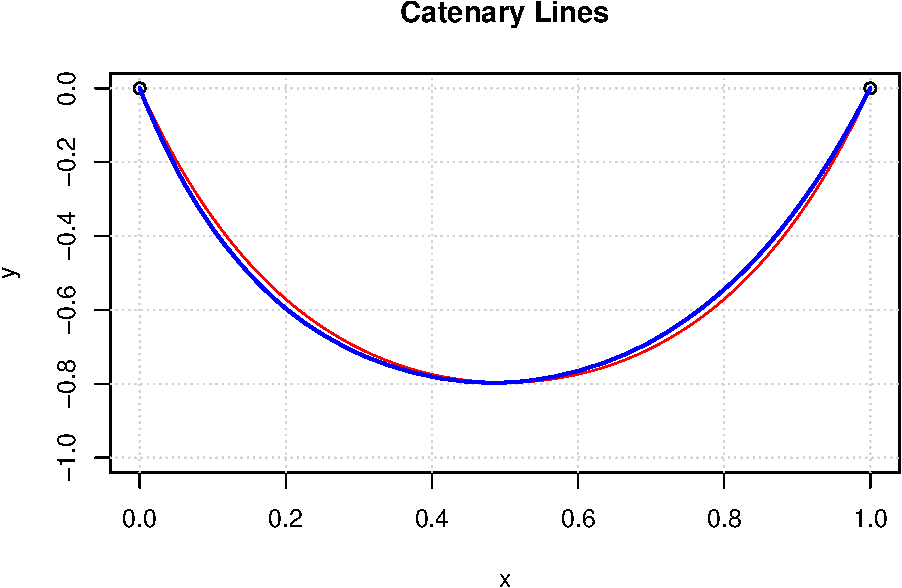
\includegraphics{catenary_files/figure-latex/unnamed-chunk-7-1.pdf}

The red curve is the solution generated by Ipopt (as a NEOS server) and
coincides with the theoretical solution \[
  f0(x) = 0.22964 \cosh(\frac{x - 0.5}{0.22964}) - 1.02603
\] The blue curve is the one generated above with \texttt{auglag} and
\texttt{optim} as internal solver. The accuracy is not perfect, but
relatively good. What is striking is that the solution is not symmetric
as should be.

\paragraph{auglag() with nlminb solver}\label{auglag-with-nlminb-solver}

Let us compare this with the other solver, that is with \texttt{nlminb}
as internal solver. Here are the results, displayed in a graph.

\begin{Shaded}
\begin{Highlighting}[]
\KeywordTok{system.time}\NormalTok{(}
\NormalTok{sol2 <-}\StringTok{ }\NormalTok{alabama::}\KeywordTok{auglag}\NormalTok{(p0, fnobj, }\DataTypeTok{hin=}\NormalTok{hin, }\DataTypeTok{heq=}\NormalTok{heq,}
                       \DataTypeTok{control.outer=}\KeywordTok{list}\NormalTok{(}\DataTypeTok{method=}\StringTok{"nlminb"}\NormalTok{, }\DataTypeTok{trace=}\OtherTok{FALSE}\NormalTok{))}
\NormalTok{)}
\end{Highlighting}
\end{Shaded}

\begin{verbatim}
##    user  system elapsed 
##  12.665   0.903  13.594
\end{verbatim}

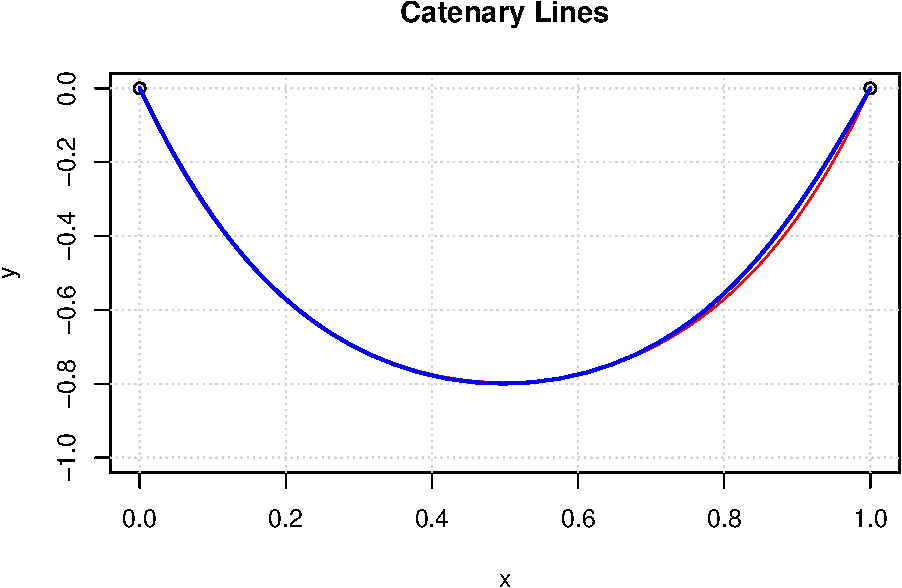
\includegraphics{catenary_files/figure-latex/unnamed-chunk-9-1.pdf}

We can see that the \texttt{nlminb} solver takes about 1.5 times longer,
but the result is more accrate, but still not accurate. I admit I was
surprised that \texttt{nlminb} worked that good.

\paragraph{optim and nlminb with 100
links}\label{optim-and-nlminb-with-100-links}

To increase accuracy, we will solve the problem again with both solver,
now with 101 points (or 100 chin links). Here I only show the results in
one graph.

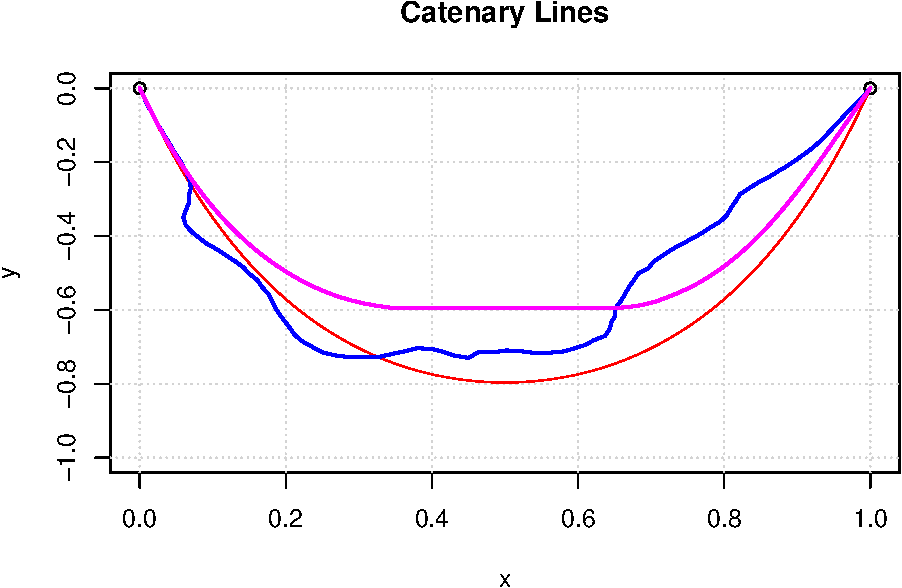
\includegraphics{catenary_files/figure-latex/unnamed-chunk-10-1.pdf}

The line in blue shows the solution with \texttt{optim}, in magenta the
solution obtained with \texttt{nlminb}. Obviously the outer loop breaks
off too early. This probably can be amended by changing outer option, it
is unclear (to me) which ones to change how.

Timings in these cases were 25-30 seconds.

\paragraph{auglag with lbfgs solver}\label{auglag-with-lbfgs-solver}

I have generated a version of \texttt{alabama::auglag} with
\texttt{lbfgs::lbfgs} as inner solver. \texttt{lbfgs()} should be more
accurate and hopefully much faster.

\begin{Shaded}
\begin{Highlighting}[]
\KeywordTok{source}\NormalTok{(}\StringTok{"auglag2.R"}\NormalTok{)}
\KeywordTok{system.time}\NormalTok{(}
    \NormalTok{sol <-}\StringTok{ }\KeywordTok{auglag_lbfgs}\NormalTok{(p0, fnobj, grobj, hin, hin.jac, heq, heq.jac)}
\NormalTok{)}
\end{Highlighting}
\end{Shaded}

\begin{verbatim}
## Warning in if (bfgs_method == "lbfgs") {: the condition has length > 1 and
## only the first element will be used

## Warning in if (bfgs_method == "lbfgs") {: the condition has length > 1 and
## only the first element will be used

## Warning in if (bfgs_method == "lbfgs") {: the condition has length > 1 and
## only the first element will be used

## Warning in if (bfgs_method == "lbfgs") {: the condition has length > 1 and
## only the first element will be used

## Warning in if (bfgs_method == "lbfgs") {: the condition has length > 1 and
## only the first element will be used

## Warning in if (bfgs_method == "lbfgs") {: the condition has length > 1 and
## only the first element will be used
\end{verbatim}

\begin{verbatim}
##    user  system elapsed 
## 160.051  10.443 170.803
\end{verbatim}

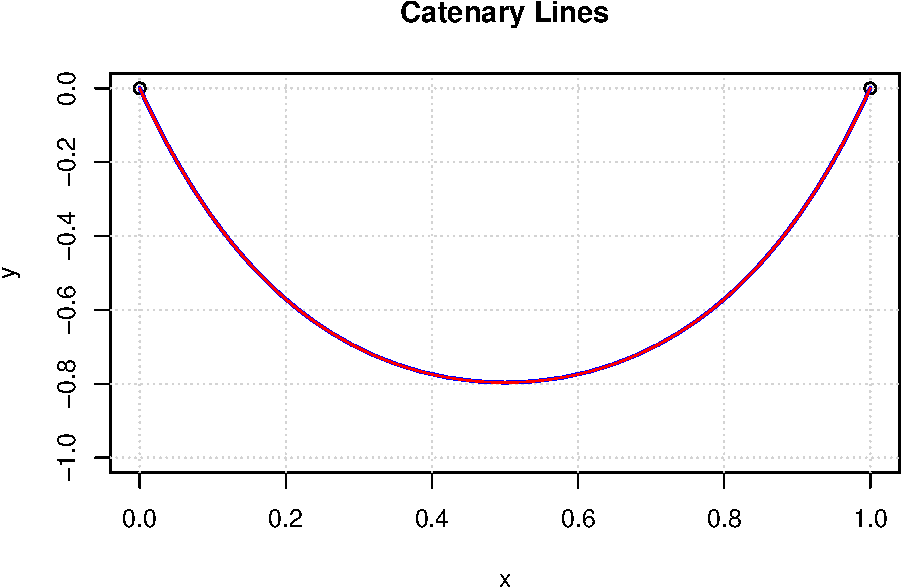
\includegraphics{catenary_files/figure-latex/unnamed-chunk-12-1.pdf}

We see that even with 50 points the result is most accurate, comparable
to the solution found by Ipopt. What is disappointing is the very long
running time. I still have to find out what actually makes it so slow.

The solution is not brittle in the sense that with 100 points the same
solution comes out, though it takes even much longer.

\paragraph{NLopt with SLSQP}\label{nlopt-with-slsqp}

It would be natural to solve the catenary problem with augmented
Lagrangian procedure \texttt{auglag()} from the \emph{nloptr} package,
either with gradient through \texttt{BFGS} or without gradients using
the \texttt{COBYLA} approach. Unfortunately, I have not been able to
call \texttt{nloptr::auglag()} correctly.

Instead I will apply the NLopt routine SLSQP directly. \texttt{slsqp()}
realizes ``sequential quadratic programming'' (SQP) and appears thus to
be specially appropriate for a problem with quadratic objective and/or
constraints.

\begin{Shaded}
\begin{Highlighting}[]
\CommentTok{# require(nloptr, quietly=TRUE)}
\KeywordTok{system.time}\NormalTok{(}
\NormalTok{sol <-}\StringTok{ }\NormalTok{nloptr::}\KeywordTok{slsqp}\NormalTok{(p0, fnobj, }\DataTypeTok{gr=}\NormalTok{grobj,}
                     \DataTypeTok{hin=}\NormalTok{hin, }\DataTypeTok{hinjac=}\NormalTok{hin.jac,}
                     \DataTypeTok{heq=}\NormalTok{heq, }\DataTypeTok{heqjac=}\NormalTok{heq.jac)}
\NormalTok{)}
\end{Highlighting}
\end{Shaded}

\begin{verbatim}
##    user  system elapsed 
##   3.696   0.208   3.914
\end{verbatim}

This solves the catenary problem as exactly as \texttt{auglag\_lbfgs()}
above, but in much less time, as can be seen from the following plot.

The solver `slsqp()' will solve the catenary problem in about 25
seconds. For decidedly more than 100 points the solver will stop working
and return the starting point.

\begin{Shaded}
\begin{Highlighting}[]
\NormalTok{x <-}\StringTok{ }\NormalTok{sol$par[}\DecValTok{1}\NormalTok{:N]; y <-}\StringTok{ }\NormalTok{sol$par[(N}\DecValTok{+1}\NormalTok{):(}\DecValTok{2}\NormalTok{*N)]}
\KeywordTok{plot}\NormalTok{(}\KeywordTok{c}\NormalTok{(}\DecValTok{0}\NormalTok{,}\DecValTok{1}\NormalTok{), }\KeywordTok{c}\NormalTok{(-}\DecValTok{1}\NormalTok{,}\DecValTok{0}\NormalTok{), }\DataTypeTok{type=}\StringTok{'n'}\NormalTok{)}
\KeywordTok{lines}\NormalTok{(x, y, }\DataTypeTok{col=}\StringTok{"blue"}\NormalTok{, }\DataTypeTok{lwd=}\DecValTok{2}\NormalTok{)}
\KeywordTok{points}\NormalTok{(}\KeywordTok{c}\NormalTok{(}\DecValTok{0}\NormalTok{, }\DecValTok{1}\NormalTok{), }\KeywordTok{c}\NormalTok{(}\DecValTok{0}\NormalTok{, }\DecValTok{0}\NormalTok{))}
\KeywordTok{curve}\NormalTok{(}\FloatTok{0.22964}\NormalTok{*}\KeywordTok{cosh}\NormalTok{((x}\FloatTok{-0.5}\NormalTok{)/}\FloatTok{0.22964}\NormalTok{)-}\FloatTok{1.02603}\NormalTok{, }\DecValTok{0}\NormalTok{, }\DecValTok{1}\NormalTok{,}
      \DataTypeTok{col=}\StringTok{"red"}\NormalTok{, }\DataTypeTok{add=}\OtherTok{TRUE}\NormalTok{)}
\KeywordTok{grid}\NormalTok{()}
\end{Highlighting}
\end{Shaded}

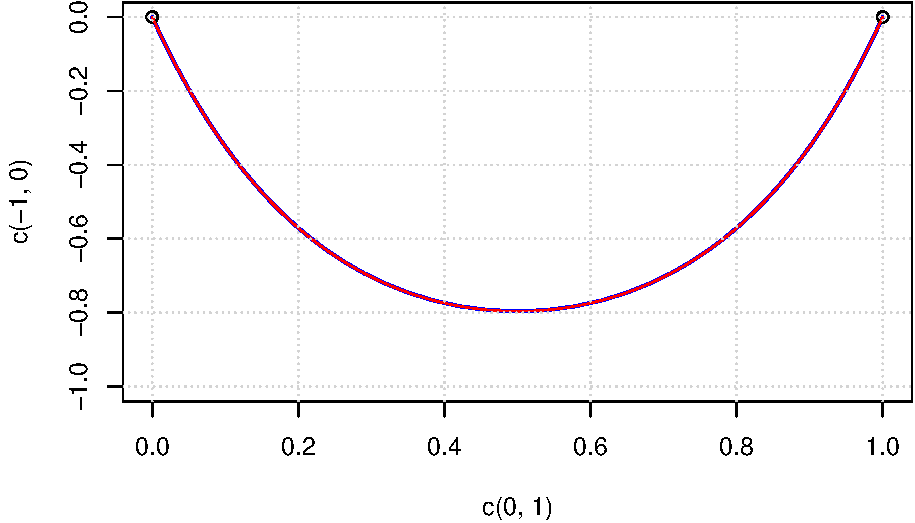
\includegraphics{catenary_files/figure-latex/unnamed-chunk-14-1.pdf}

By the way: Trying to utilize packages `Rsolnp' or `NlcOptim' was
entirely in vain. The results were either completely wrong or returned
simply the starting point. Probably calling the procedures was done
incorrectly, though I was unable to identify a correct call in several
tries.

\subsubsection{\texorpdfstring{The `conic programming'
approach}{The conic programming approach}}\label{the-conic-programming-approach}

\paragraph{\texorpdfstring{Solving the catenary with
\emph{ECOSolveR}}{Solving the catenary with ECOSolveR}}\label{solving-the-catenary-with-ecosolver}

The catenary problem is formulated as a linear objective with quadratic
constraints, QCLP. As there are no linear solvers with such constraints,
the next step up would be to handle it as quadratic with quadratic
constraints, QCQP. Quadratic solvers in R do not allow for quadratic
constraints, so the next logical step is solving it as a convex problem
with convex constraints.

A quite powerful solver for these kinds of problems is ECOS, an embedded
conic solver, integrated with R in the \emph{ECOSolver} package. Using
the interface of \emph{ECOSolver} can get quite complicated. Stephen
Boyd and colleagues are building another package \emph{cvxr} that will
define an optimization modeling language, maybe a bit similar to Julia's
\emph{JuMP} module.

\begin{Shaded}
\begin{Highlighting}[]
\KeywordTok{require}\NormalTok{(Matrix, }\DataTypeTok{quietly=}\OtherTok{TRUE}\NormalTok{)}
\KeywordTok{require}\NormalTok{(ECOSolveR, }\DataTypeTok{quietly=}\OtherTok{TRUE}\NormalTok{)}

\NormalTok{N <-}\StringTok{ }\DecValTok{51}                 \CommentTok{# 2N + 1 variables}
\NormalTok{L <-}\StringTok{ }\DecValTok{1}\NormalTok{; h <-}\StringTok{ }\DecValTok{2}\NormalTok{/(N}\DecValTok{-1}\NormalTok{)}
\end{Highlighting}
\end{Shaded}

We will add one more variable \(x_0\) resp. \(x_{2N+1}\) to the
coordinates in order to be able to define the conic inequality
constraints. Therefore, the objective function is

\begin{Shaded}
\begin{Highlighting}[]
\NormalTok{c <-}\StringTok{ }\KeywordTok{c}\NormalTok{(}\KeywordTok{rep}\NormalTok{(}\DecValTok{0}\NormalTok{,N), }\KeywordTok{rep}\NormalTok{(}\DecValTok{1}\NormalTok{,N), }\DecValTok{0}\NormalTok{)}
\end{Highlighting}
\end{Shaded}

The extra variable will have a fixed value of \(h\). Together with
fixing the left and right end points of the chain we can define the
following \emph{sparse} matrix \(A\) and RHS \(b\):

\begin{Shaded}
\begin{Highlighting}[]
\NormalTok{A <-}\StringTok{ }\KeywordTok{Matrix}\NormalTok{(}\DecValTok{0}\NormalTok{, }\DataTypeTok{nrow=}\DecValTok{5}\NormalTok{, }\DataTypeTok{ncol=}\DecValTok{2}\NormalTok{*N}\DecValTok{+1}\NormalTok{, }\DataTypeTok{sparse=}\OtherTok{TRUE}\NormalTok{)}
\NormalTok{A[}\DecValTok{1}\NormalTok{, }\DecValTok{2}\NormalTok{*N}\DecValTok{+1}\NormalTok{] <-}\StringTok{ }\DecValTok{1}                \CommentTok{# x[2*N+1] = 1}
\NormalTok{A[}\DecValTok{2}\NormalTok{, }\DecValTok{1}\NormalTok{] <-}\StringTok{ }\DecValTok{1}\NormalTok{; A[}\DecValTok{3}\NormalTok{, N] <-}\StringTok{ }\DecValTok{1}      \CommentTok{# x[1] = 0; x[N] = 1}
\NormalTok{A[}\DecValTok{4}\NormalTok{, N}\DecValTok{+1}\NormalTok{] <-}\StringTok{ }\DecValTok{1}\NormalTok{; A[}\DecValTok{5}\NormalTok{, }\DecValTok{2}\NormalTok{*N] <-}\StringTok{ }\DecValTok{1}  \CommentTok{# y[1] = 1; y[N] = 1}

\NormalTok{b =}\StringTok{ }\KeywordTok{c}\NormalTok{(h, }\DecValTok{0}\NormalTok{, }\DecValTok{1}\NormalTok{, }\DecValTok{1}\NormalTok{, }\DecValTok{1}\NormalTok{)}
\end{Highlighting}
\end{Shaded}

The inequality constraints are all of the form
\((x_{i+1}-x_i)^2 + (y_{i+1}-y_i)^2 \le h\). For a ``conic formulation''
we need a linear functional \(G_i\) such that (remember,
\(y_i = x_{N+i}\)) \[
    G_i(x) = (h, x_{i+1}-x_i, x_{N+i+1}-x_{N+i}) = (h, X) \in K
\] as being an element of cone \(K\) means \(h \ge ||X||_2\) -- or: the
\(i\)-th chain link is smaller than \(h\). The following \emph{sparse}
matrix \(G\) defines \(N-1\) such submatrices \(G_i\), each three rows
ans \(2N+1\) columns.

\begin{Shaded}
\begin{Highlighting}[]
\NormalTok{G <-}\StringTok{ }\KeywordTok{Matrix}\NormalTok{(}\DecValTok{0}\NormalTok{, }\DataTypeTok{nrow=}\DecValTok{3}\NormalTok{*(N}\DecValTok{-1}\NormalTok{), }\DataTypeTok{ncol=}\DecValTok{2}\NormalTok{*N}\DecValTok{+1}\NormalTok{, }\DataTypeTok{sparse=}\OtherTok{TRUE}\NormalTok{)}

\NormalTok{for (i in }\DecValTok{1}\NormalTok{:(N}\DecValTok{-1}\NormalTok{)) \{}
    \NormalTok{j <-}\StringTok{ }\DecValTok{3}\NormalTok{*(i}\DecValTok{-1}\NormalTok{) +}\StringTok{ }\DecValTok{1}
    \NormalTok{G[j, }\DecValTok{2}\NormalTok{*N}\DecValTok{+1}\NormalTok{] <-}\StringTok{ }\NormalTok{-}\DecValTok{1}
    \NormalTok{G[j}\DecValTok{+1}\NormalTok{, i] <-}\StringTok{ }\NormalTok{-}\DecValTok{1}\NormalTok{; G[j}\DecValTok{+1}\NormalTok{, i}\DecValTok{+1}\NormalTok{] <-}\StringTok{ }\DecValTok{1}
    \NormalTok{G[j}\DecValTok{+2}\NormalTok{, N+i] <-}\StringTok{ }\NormalTok{-}\DecValTok{1}\NormalTok{; G[j}\DecValTok{+2}\NormalTok{, N+i}\DecValTok{+1}\NormalTok{] <-}\StringTok{ }\DecValTok{1}
\NormalTok{\}}
\end{Highlighting}
\end{Shaded}

In the conic formulation \(G_i(x) \le{}_K h\) we do not need the \(h\)s,
so the right hand side is:

\begin{Shaded}
\begin{Highlighting}[]
\NormalTok{H <-}\StringTok{ }\KeywordTok{rep}\NormalTok{(}\DecValTok{0}\NormalTok{, }\DecValTok{3}\NormalTok{*(N}\DecValTok{-1}\NormalTok{))}
\end{Highlighting}
\end{Shaded}

and as each three rows belong together, the \texttt{dims} argument is:

\begin{Shaded}
\begin{Highlighting}[]
\NormalTok{quad <-}\StringTok{ }\KeywordTok{as.integer}\NormalTok{(}\KeywordTok{rep}\NormalTok{(}\DecValTok{3}\NormalTok{, N}\DecValTok{-1}\NormalTok{))}
\end{Highlighting}
\end{Shaded}

Now we have gathered all puzzle pieces and call the ECOS solver:

\begin{Shaded}
\begin{Highlighting}[]
\KeywordTok{system.time}\NormalTok{(}
  \NormalTok{sole <-}\StringTok{ }\KeywordTok{ECOS_csolve}\NormalTok{(c, G, H, }\DataTypeTok{dims=}\KeywordTok{list}\NormalTok{(}\DataTypeTok{q=}\NormalTok{quad), A, b)}
\NormalTok{)}
\end{Highlighting}
\end{Shaded}

\begin{verbatim}
##    user  system elapsed 
##   0.002   0.000   0.003
\end{verbatim}

The solution exactly follows the theoretical solution (the red line).

\begin{Shaded}
\begin{Highlighting}[]
\NormalTok{xs <-}\StringTok{ }\NormalTok{sole$x[}\DecValTok{1}\NormalTok{:N]; ys <-}\StringTok{ }\NormalTok{sole$x[(N}\DecValTok{+1}\NormalTok{):(}\DecValTok{2}\NormalTok{*N)]}
\KeywordTok{plot}\NormalTok{(}\KeywordTok{c}\NormalTok{(}\DecValTok{0}\NormalTok{, }\DecValTok{1}\NormalTok{), }\KeywordTok{c}\NormalTok{(}\DecValTok{0}\NormalTok{, }\DecValTok{1}\NormalTok{), }\DataTypeTok{type=}\StringTok{'n'}\NormalTok{)}
\KeywordTok{lines}\NormalTok{(xs, ys, }\DataTypeTok{col=}\StringTok{"blue"}\NormalTok{, }\DataTypeTok{lwd=}\DecValTok{2}\NormalTok{)}

\KeywordTok{points}\NormalTok{(}\KeywordTok{c}\NormalTok{(}\DecValTok{0}\NormalTok{, }\DecValTok{1}\NormalTok{), }\KeywordTok{c}\NormalTok{(}\DecValTok{1}\NormalTok{, }\DecValTok{1}\NormalTok{))}
\KeywordTok{curve}\NormalTok{(}\FloatTok{0.22964}\NormalTok{*}\KeywordTok{cosh}\NormalTok{((x}\FloatTok{-0.5}\NormalTok{)/}\FloatTok{0.22964}\NormalTok{)-}\FloatTok{0.02603}\NormalTok{, }\DecValTok{0}\NormalTok{, }\DecValTok{1}\NormalTok{,}
      \DataTypeTok{col=}\StringTok{"red"}\NormalTok{, }\DataTypeTok{add=}\OtherTok{TRUE}\NormalTok{)}
\KeywordTok{grid}\NormalTok{()}
\end{Highlighting}
\end{Shaded}

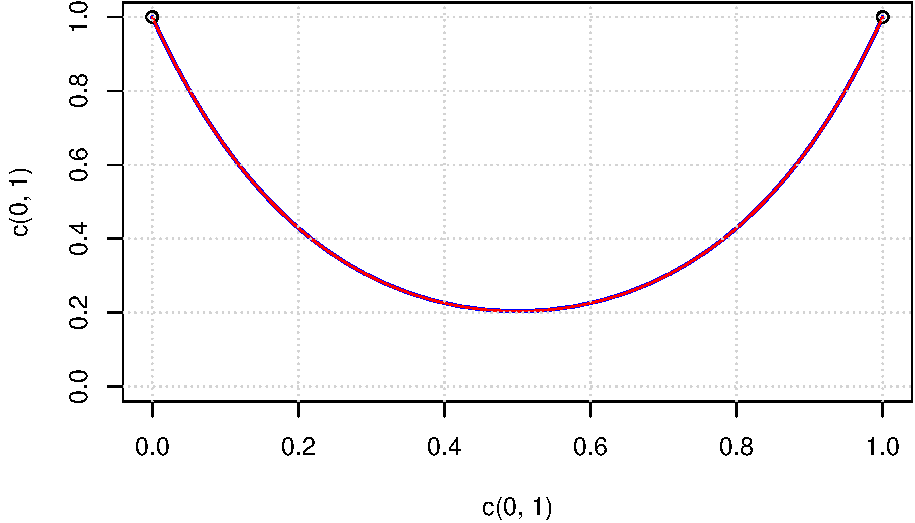
\includegraphics{catenary_files/figure-latex/unnamed-chunk-22-1.pdf}

The timings are 2/3/36 milliseconds for 50/100/1000 chain links.

\paragraph{\texorpdfstring{Solving the catenary with
\emph{SCS}}{Solving the catenary with SCS}}\label{solving-the-catenary-with-scs}

SCS (Conic Splitting Solver) is another of the solvers developed by
Stephen Boyd and colleagues at Stanford University. An R interface is
available in the \emph{scs} package maintained by Florian Schwendinger.

The API of \texttt{scs()} is similar to that one for
\texttt{ECOS\_csolve()} except that the matrices \texttt{A} and
\texttt{G} are combined into one, and then necessarily also \texttt{b}
and \texttt{h}. So with all the (sparse) matrices and vectors defined in
the section on the \emph{ECOSolveR} package we can call \texttt{scs()}
in just one line.

\begin{Shaded}
\begin{Highlighting}[]
\KeywordTok{library}\NormalTok{(scs)}
\KeywordTok{system.time}\NormalTok{(}
\NormalTok{sol_scs <-}\StringTok{ }\KeywordTok{scs}\NormalTok{(}\DataTypeTok{A=}\KeywordTok{rbind}\NormalTok{(A, G), }\DataTypeTok{b=}\KeywordTok{c}\NormalTok{(b, H), }\DataTypeTok{obj=}\NormalTok{c, }\DataTypeTok{cone=}\KeywordTok{list}\NormalTok{(}\DataTypeTok{f=}\KeywordTok{nrow}\NormalTok{(A), }\DataTypeTok{q=}\NormalTok{quad))}
\NormalTok{)}
\end{Highlighting}
\end{Shaded}

\begin{verbatim}
##    user  system elapsed 
##   0.004   0.000   0.004
\end{verbatim}

\begin{Shaded}
\begin{Highlighting}[]
\KeywordTok{str}\NormalTok{(sol_scs)}
\end{Highlighting}
\end{Shaded}

\begin{verbatim}
## List of 4
##  $ x   : num [1:103] 1.16e-07 9.13e-03 1.86e-02 2.85e-02 3.88e-02 ...
##  $ y   : num [1:155] 712.94 5.74 -5.74 -25.5 -25.5 ...
##  $ s   : num [1:155] 4.14e-15 -8.60e-18 6.22e-18 7.42e-17 -5.77e-17 ...
##  $ info:List of 12
##   ..$ iter     : int 320
##   ..$ status   : chr "Solved"
##   ..$ statusVal: int 1
##   ..$ pobj     : num 28.2
##   ..$ dobj     : num 28.2
##   ..$ resPri   : num 6.38e-07
##   ..$ resDual  : num 7.48e-07
##   ..$ resInfeas: num 0.438
##   ..$ resUnbdd : num NaN
##   ..$ relGap   : num 2.45e-08
##   ..$ setupTime: num 0.0979
##   ..$ solveTime: num 1.84
\end{verbatim}

The timings for \emph{scs} are 2/10/280 for 50/100/1000 links. The RMS
error (`root mean square error') for 50 links is 0.0001514347 compared
to 0.0001508338 for ECOS.

\paragraph{\texorpdfstring{Solving the catenary with
\emph{Rmosek}}{Solving the catenary with Rmosek}}\label{solving-the-catenary-with-rmosek}

MOSEK is an interior-point solver for large-scale optimization problems.
MOSEK is capable of efficiently solving LP, QP, SOCP, and SDP problems.
MOSEK is commercial, but there are academic licenses available.

Package \emph{Rmosek} provides an R interface for the MOSEK program if
MOSEK itself is already installed on the system. Setting up a problem in
a form appropriate for sending it to MOSEK is still quite complicated as
can be seen from the following code handling the catenary problem for
\emph{Rmosek} and MOSEK.

\begin{Shaded}
\begin{Highlighting}[]
\KeywordTok{require}\NormalTok{(Matrix, }\DataTypeTok{quietly=}\OtherTok{TRUE}\NormalTok{)}
\KeywordTok{require}\NormalTok{(Rmosek, }\DataTypeTok{quietly=}\OtherTok{TRUE}\NormalTok{)}

\NormalTok{N <-}\StringTok{ }\DecValTok{51}                 \CommentTok{# 2N + 2N-2 + N-1 variables}
\NormalTok{L <-}\StringTok{ }\DecValTok{1}\NormalTok{; h <-}\StringTok{ }\DecValTok{2}\NormalTok{/(N}\DecValTok{-1}\NormalTok{)}

\CommentTok{# model list cp with cp$c the linear objective}
\NormalTok{cp <-}\StringTok{ }\KeywordTok{list}\NormalTok{(}\DataTypeTok{sense=}\StringTok{"min"}\NormalTok{) }\CommentTok{# minimization problem}
\NormalTok{cp$c <-}\StringTok{ }\KeywordTok{c}\NormalTok{(}\KeywordTok{rep}\NormalTok{(}\DecValTok{0}\NormalTok{,N), }\KeywordTok{rep}\NormalTok{(}\DecValTok{1}\NormalTok{,N), }\KeywordTok{rep}\NormalTok{(}\DecValTok{0}\NormalTok{,}\DecValTok{3}\NormalTok{*N}\DecValTok{-3}\NormalTok{))}

\CommentTok{# sparse matrix defining the differences x_i - x_\{i+1\}}
\NormalTok{A <-}\StringTok{ }\KeywordTok{Matrix}\NormalTok{(}\DecValTok{0}\NormalTok{, }\DataTypeTok{nrow=}\DecValTok{2}\NormalTok{*N}\DecValTok{-2}\NormalTok{, }\DataTypeTok{ncol=}\DecValTok{5}\NormalTok{*N}\DecValTok{-3}\NormalTok{, }\DataTypeTok{sparse=}\OtherTok{TRUE}\NormalTok{)}
\NormalTok{for (i in }\DecValTok{1}\NormalTok{:(N}\DecValTok{-1}\NormalTok{)) \{}
    \NormalTok{A[i,i] <-}\StringTok{ }\DecValTok{1}\NormalTok{; A[i,i}\DecValTok{+1}\NormalTok{] <-}\StringTok{ }\NormalTok{-}\DecValTok{1}\NormalTok{; A[i,}\DecValTok{2}\NormalTok{*N+i] <-}\StringTok{ }\DecValTok{1}
    \NormalTok{A[N}\DecValTok{-1}\NormalTok{+i,N+i] <-}\StringTok{ }\DecValTok{1}\NormalTok{; A[N}\DecValTok{-1}\NormalTok{+i,N+i}\DecValTok{+1}\NormalTok{] <-}\StringTok{ }\NormalTok{-}\DecValTok{1}\NormalTok{; A[N}\DecValTok{-1}\NormalTok{+i,}\DecValTok{3}\NormalTok{*N}\DecValTok{-1}\NormalTok{+i] <-}\StringTok{ }\DecValTok{1}
\NormalTok{\}}
\NormalTok{cp$A <-}\StringTok{ }\NormalTok{A}

\CommentTok{# rhs of the linear equalities defined through matrix A}
\NormalTok{cp$bc <-}\StringTok{ }\KeywordTok{rbind}\NormalTok{(}\DataTypeTok{blc=}\KeywordTok{rep}\NormalTok{(}\DecValTok{0}\NormalTok{,}\DecValTok{2}\NormalTok{*N}\DecValTok{-2}\NormalTok{), }\DataTypeTok{buc=}\KeywordTok{rep}\NormalTok{(}\DecValTok{0}\NormalTok{,}\DecValTok{2}\NormalTok{*N}\DecValTok{-2}\NormalTok{))}

\CommentTok{# bounds on the free variables}
\NormalTok{cp$bx <-}\StringTok{ }\KeywordTok{rbind}\NormalTok{(}\DataTypeTok{blx=}\KeywordTok{c}\NormalTok{(}\DecValTok{0}\NormalTok{,}\KeywordTok{rep}\NormalTok{(-}\OtherTok{Inf}\NormalTok{,N}\DecValTok{-2}\NormalTok{),}\DecValTok{1}\NormalTok{,}\DecValTok{0}\NormalTok{,}\KeywordTok{rep}\NormalTok{(-}\OtherTok{Inf}\NormalTok{,N}\DecValTok{-2}\NormalTok{),}\DecValTok{0}\NormalTok{,}\KeywordTok{rep}\NormalTok{(-}\OtherTok{Inf}\NormalTok{,}\DecValTok{2}\NormalTok{*N}\DecValTok{-2}\NormalTok{),}\KeywordTok{rep}\NormalTok{(h,N}\DecValTok{-1}\NormalTok{)),}
               \DataTypeTok{bux=}\KeywordTok{c}\NormalTok{(}\DecValTok{0}\NormalTok{,}\KeywordTok{rep}\NormalTok{( }\OtherTok{Inf}\NormalTok{,N}\DecValTok{-2}\NormalTok{),}\DecValTok{1}\NormalTok{,}\DecValTok{0}\NormalTok{,}\KeywordTok{rep}\NormalTok{( }\OtherTok{Inf}\NormalTok{,N}\DecValTok{-2}\NormalTok{),}\DecValTok{0}\NormalTok{,}\KeywordTok{rep}\NormalTok{( }\OtherTok{Inf}\NormalTok{,}\DecValTok{2}\NormalTok{*N}\DecValTok{-2}\NormalTok{),}\KeywordTok{rep}\NormalTok{(h,N}\DecValTok{-1}\NormalTok{)))}

\CommentTok{# define the cones h >= ||(x_i-x_\{i+1\})^2 + (y_i-y_\{i+1\})^2||}
\NormalTok{co <-}\StringTok{ }\KeywordTok{cbind}\NormalTok{(}\KeywordTok{list}\NormalTok{(}\StringTok{"QUAD"}\NormalTok{, }\KeywordTok{c}\NormalTok{(}\DecValTok{4}\NormalTok{*N}\DecValTok{-2+1}\NormalTok{, }\DecValTok{2}\NormalTok{*N}\DecValTok{+1}\NormalTok{, }\DecValTok{3}\NormalTok{*N)))}
\NormalTok{for (i in }\DecValTok{2}\NormalTok{:(N}\DecValTok{-1}\NormalTok{)) \{}
    \NormalTok{co <-}\StringTok{ }\KeywordTok{cbind}\NormalTok{(co, }\KeywordTok{list}\NormalTok{(}\StringTok{"QUAD"}\NormalTok{, }\KeywordTok{c}\NormalTok{(}\DecValTok{4}\NormalTok{*N}\DecValTok{-2}\NormalTok{+i, }\DecValTok{2}\NormalTok{*N+i, }\DecValTok{3}\NormalTok{*N}\DecValTok{-1}\NormalTok{+i)))}
\NormalTok{\}}
\NormalTok{cp$cones <-}\StringTok{ }\NormalTok{co}

\KeywordTok{system.time}\NormalTok{(r <-}\StringTok{ }\KeywordTok{mosek}\NormalTok{(cp, }\DataTypeTok{opts=}\KeywordTok{list}\NormalTok{(}\DataTypeTok{verbose=}\DecValTok{1}\NormalTok{)))}
\end{Highlighting}
\end{Shaded}

\begin{verbatim}
##    user  system elapsed 
##   0.015   0.002   0.016
\end{verbatim}

Plotting the solution \texttt{r\$sol\$itr\$xx} against the theoretical
solution as above generates the the same plots as above. MOSEK solves
the catenary problem with 50/100/1000 points in 4/5/33 microseconds.

\subsubsection{Appendices (Solving it outside
R)}\label{appendices-solving-it-outside-r}

\paragraph{Appendix: Julia and ECOS}\label{appendix-julia-and-ecos}

The Julia `ECOS.jl' package provides a wrapper for the interior-point
solver ECOS for second-order cone problems. And `JuMP' provides a
domain-specific modeling language for optimization problems in Julia. It
can apply commercial and open source solvers.

The following is a formulation of the catenary problem in JuMP, calling
ECOS as conic solver. A correct and highly accurate result is returned
within 0.0065/0.0157/0.4158 seconds for 50/100/1000 points.

\begin{verbatim}
using JuMP
using ECOS

n = 51
L = 2; h = L/(n-1)

m = Model(solver=ECOSSolver())

@variable(m, x[1:(2*n)] >= 0.0)
@objective(m, Min, sum{x[i], i=(n+1):(2*n)})

@constraints(m, begin
  x[1]   == 0; x[n]   == 1
  x[n+1] == 1; x[2*n] == 1
end)

for i in 1:(n-1)
    A = zeros(2, 2*n)
    A[1, i] = -1; A[1, i+1] = 1
    A[2, n+i] = -1; A[2, n+i+1] = 1
    @constraint(m, soc, norm(A*x) <= h)
end

status = solve(m)
\end{verbatim}

\paragraph{Appendix: Problem Formulation in
AMPL}\label{appendix-problem-formulation-in-ampl}

\begin{verbatim}
param N := 100; # number of chainlinks
param L := 1;   # difference in x-coords of endlinks

param h := 2*L/N;   # length of each link

var x {0..N};   # x-coordinates of endpoints of chainlinks
var y {0..N};   # y-coordinates of endpoints of chainlinks

minimize pot_energy: sum{j in 1..N} (y[j-1] + y[j])/2;

subject to x_left_anchor: x[0] = 0;
subject to y_left_anchor: y[0] = 0;
subject to x_right_anchor: x[N] = L;
subject to y_right_anchor: y[N] = 0;

subject to link_up {j in 1..N}: (x[j] - x[j-1])^2 + (y[j] - y[j-1])^2 <= h^2;

let {j in 0..N} x[j] := j*L/N;
let {j in 0..N} y[j] := 0;

solve;

printf {j in 0..N}: "%10.5f %10.5f \n", x[j], y[j]
\end{verbatim}


\end{document}
